\documentclass{csbeamer}

\usepackage{dsfont}
\usepackage{amsmath}
\usepackage{amssymb}
\usepackage{algorithm}
\usepackage{algpseudocode}
\usepackage{pgfplots}
\usepackage{colortbl}
\usepackage{xcolor}
\pgfplotsset{compat=1.18}

% Add custom color definitions for TD Learning
\definecolor{tdmain}{HTML}{2E7D32}
\definecolor{tdaccent}{HTML}{FF6F00}
\definecolor{tdlight}{HTML}{66BB6A}
\definecolor{tdsecondary}{HTML}{3F51B5}
\definecolor{tdeval}{HTML}{9C27B0}
\definecolor{tdimprove}{HTML}{E91E63}
\definecolor{tdvalue}{HTML}{FF9800}
\definecolor{tdpolicy}{HTML}{795548}
\definecolor{tdonpolicy}{HTML}{388E3C}
\definecolor{tdoffpolicy}{HTML}{5D4037}
\definecolor{tdactivity}{HTML}{1976D2}
\definecolor{tderror}{HTML}{D32F2F}

\university{St. Francis Xavier University}
\department{Department of Computer Science}
\course{CSCI-531 - Reinforcement Learning}
\courseshort{CSCI-531 - RL}
\term{Fall 2025}
\author{Dr. Jean-Alexis Delamer}

\title{Temporal-Difference Learning}

\begin{document}

\frame{\titlepage}

% Section: Introduction
\section{Introduction}

\subsection{Bridging DP and Monte Carlo}

\begin{frame}
    \frametitle{The Best of Both Worlds}

    \begin{block}<1->{What is Temporal-Difference Learning?}
        \begin{itemize}
            \item<1-> Combines \textcolor{tdmain}{\textbf{Dynamic Programming}} and \textcolor{tdaccent}{\textbf{Monte Carlo}} methods
            \item<2-> \textcolor{tdsecondary}{\textbf{Model-free}} like Monte Carlo
            \item<3-> \textcolor{tdlight}{\textbf{Bootstraps}} like Dynamic Programming
        \end{itemize}
    \end{block}

    \begin{block}<4->{Key Insight}
        \begin{itemize}
            \item<4-> Updates estimates based on \textcolor{tdmain}{\textbf{other estimates}}
            \item<5-> No need to wait until episode completion
            \item<6-> Updates at \textcolor{tdaccent}{\textbf{every time step}}
        \end{itemize}
    \end{block}
\end{frame}

\begin{frame}
    \frametitle{Method Comparison}

    \begin{center}
        \begin{tabular}{|l|c|c|c|}
            \hline
            \textbf{Method} & \textbf{Model-Free} & \textbf{Bootstraps} & \textbf{Online} \\
            \hline
            \rowcolor{gray!20}
            Dynamic Programming & \textcolor{red}{No} & \textcolor{green}{Yes} & \textcolor{green}{Yes} \\
            \hline
            Monte Carlo & \textcolor{green}{Yes} & \textcolor{red}{No} & \textcolor{red}{No} \\
            \hline
            \rowcolor{tdlight!30}
            \textbf{TD Learning} & \textcolor{green}{\textbf{Yes}} & \textcolor{green}{\textbf{Yes}} & \textcolor{green}{\textbf{Yes}} \\
            \hline
        \end{tabular}
    \end{center}
    \begin{block}<2->{Why This Matters}
        \begin{itemize}
            \item<2-> Can learn from \textcolor{tdmain}{\textbf{incomplete episodes}}
            \item<3-> Faster convergence than Monte Carlo
            \item<4-> More practical for \textcolor{tdaccent}{\textbf{online learning}}
        \end{itemize}
    \end{block}
\end{frame}

% Section: TD Prediction
\section{TD Prediction}

\subsection{The TD Update Rule}

\begin{frame}
    \frametitle{Activity: Monte Carlo Limitation}

    \begin{block}{Recall: Monte Carlo Update}
        \begin{center}
            \includegraphics[width=0.6\textwidth]{MC_update.png}
        \end{center}
    \end{block}
    \begin{block}{Question}
        \textcolor{tdactivity}{\textbf{What is the main disadvantage of this approach?}}
    \end{block}
\end{frame}

\begin{frame}
    \frametitle{Monte Carlo Limitations}

    \begin{block}{Answer: Key Disadvantages}
        \begin{itemize}
            \item<1-> Must wait until \textcolor{red}{\textbf{episode completion}}
            \item<2-> Cannot learn from \textcolor{tdaccent}{\textbf{partial episodes}}
            \item<3-> Updates are \textcolor{tderror}{\textbf{delayed}}
            \item<4-> Not suitable for \textcolor{tdvalue}{\textbf{continuing tasks}}
        \end{itemize}
    \end{block}

    \begin{block}<5->{Impact}
        \begin{itemize}
            \item<5-> Slow learning in long episodes
            \item<6-> Cannot handle infinite episodes
            \item<7-> Memory grows with episode length
        \end{itemize}
    \end{block}
\end{frame}

\begin{frame}
    \frametitle{Building the TD Update: What Do We Want?}

    \begin{block}<1->{Recall: Value Function Definition}
        \begin{equation}
            V(s) = \mathbb{E}[G_t | S_t = s] = \mathbb{E}[R_{t+1} + \gamma G_{t+1} | S_t = s]
        \end{equation}
    \end{block}

    \begin{block}<2->{Breaking Down the Return}
        \begin{align}
            V(s) &= \mathbb{E}[R_{t+1} + \gamma G_{t+1} | S_t = s]\\
            &= \mathbb{E}[R_{t+1} | S_t = s] + \gamma \mathbb{E}[G_{t+1} | S_t = s]\\
            &= \mathbb{E}[R_{t+1} | S_t = s] + \gamma \mathbb{E}[V(S_{t+1}) | S_t = s]
        \end{align}
    \end{block}

    \begin{block}<3->{The Key Insight}
        \textcolor{tdmain}{\textbf{The future return}} $G_{t+1}$ \textcolor{tdmain}{\textbf{starting from}} $S_{t+1}$ \textcolor{tdmain}{\textbf{is just}} $V(S_{t+1})$!
    \end{block}
\end{frame}

\begin{frame}
    \frametitle{From Theory to Practice: The Approximation}

    \begin{block}<1->{What We Have (Theory)}
        \begin{equation}
            V(s) = \mathbb{E}[R_{t+1} + \gamma V(S_{t+1}) | S_t = s]
        \end{equation}
    \end{block}

    \begin{block}<2->{What We Can Observe (Practice)}
        \begin{itemize}
            \item<2-> We see actual reward: $r_{t+1}$ (sample of $R_{t+1}$)
            \item<3-> We see next state: $s_{t+1}$ (sample of $S_{t+1}$)
            \item<4-> We have current estimate: $V(s_{t+1})$
        \end{itemize}
        \end{block}

    \begin{block}<5->{The Approximation}
        \begin{equation}
            \textcolor{tdaccent}{\mathbf{r_{t+1} + \gamma V(s_{t+1})}} \text{ is our estimate of } V(s_t)
        \end{equation}
    \end{block}

    \begin{block}<6->{Problem}
        But we already have an estimate $V(s_t)$! \textcolor{tderror}{\textbf{Which one to believe?}}
    \end{block}
    \end{frame}

\begin{frame}
    \frametitle{Resolving the Conflict: Learning from Error}

    \begin{block}<1->{Two Estimates of $V(s_t)$}
        \begin{itemize}
            \item<1-> \textcolor{tdvalue}{\textbf{Old estimate}}: $V(s_t)$ (what we thought before)
            \item<2-> \textcolor{tdaccent}{\textbf{New evidence}}: $r_{t+1} + \gamma V(s_{t+1})$ (what we observe)
        \end{itemize}
        \end{block}

    \begin{block}<3->{The Error}
        \begin{equation}
            \textcolor{tderror}{\delta_t} = \underbrace{r_{t+1} + \gamma V(s_{t+1})}_{\text{new evidence}} - \underbrace{V(s_t)}_{\text{old estimate}}
        \end{equation}
    \end{block}

    \begin{block}<4->{Learning Rule}
        \textcolor{tdmain}{\textbf{Move our estimate towards the new evidence:}}
        \begin{equation}
            V(s_t)^{\text{new}} = V(s_t)^{\text{old}} + \alpha \times \textcolor{tderror}{\delta_t}
        \end{equation}
        where $\alpha$ controls how much we trust the new evidence.
    \end{block}
\end{frame}

\begin{frame}
    \frametitle{The Complete TD Update Rule}

    \begin{block}<1->{Putting It All Together}
        \begin{equation}
            V(s_t) \leftarrow V(s_t) + \alpha\left[ r_{t+1} + \gamma V(s_{t+1}) - V(s_t) \right]
        \end{equation}
    \end{block}

    \begin{block}<2->{Components Explained}
        \begin{itemize}
            \item<2-> $\alpha \in [0,1]$: \textcolor{tdmain}{\textbf{learning rate}} (how much to change)
            \item<3-> $r_{t+1} + \gamma V(s_{t+1})$: \textcolor{tdaccent}{\textbf{TD target}} (new evidence)
            \item<4-> $r_{t+1} + \gamma V(s_{t+1}) - V(s_t)$: \textcolor{tderror}{\textbf{TD error}} (how wrong we were)
        \end{itemize}
    \end{block}

    \begin{block}<5->{Intuition}
        \begin{itemize}
            \item<5-> If error is \textcolor{tdmain}{\textbf{positive}}: our estimate was too low → increase it
            \item<6-> If error is \textcolor{tderror}{\textbf{negative}}: our estimate was too high → decrease it
            \item<7-> If error is \textcolor{gray}{\textbf{zero}}: our estimate was perfect → no change
        \end{itemize}
    \end{block}
\end{frame}

\begin{frame}
    \frametitle{Why This Works: The Bootstrap Principle}

    \begin{block}<1->{Bootstrap Analogy}
        \textcolor{tdmain}{\textbf{"Pulling yourself up by your bootstraps"}}
        \begin{itemize}
            \item<1-> Use current estimates to improve current estimates
            \item<2-> Like improving a recipe by tasting and adjusting as you cook
            \item<3-> Don't wait for the final dish (complete episode)
        \end{itemize}
    \end{block}

    \begin{block}<4->{Mathematical Justification}
        \begin{itemize}
            \item<4-> Each update moves us \textcolor{tdaccent}{\textbf{closer}} to the true value
            \item<5-> Estimates \textcolor{tdlight}{\textbf{propagate}} through the state space
            \item<6-> Converges to optimal values under mild conditions
        \end{itemize}
    \end{block}

    \begin{block}<7->{Key Insight}
        \textcolor{tdsecondary}{\textbf{We don't need perfect information}} - just better information than what we had!
    \end{block}
\end{frame}

\begin{frame}
    \frametitle{Visual Comparison: MC vs TD}

    \begin{center}
        \includegraphics[width=0.55\textwidth]{TD_update.png}
    \end{center}
    \begin{block}<2->{Key Differences}
        \begin{itemize}
            \item<2-> \textbf{MC}: Uses actual return $G_t$
            \item<3-> \textbf{TD}: Uses estimated return $r_{t+1} + \gamma V(s_{t+1})$
            \item<4-> \textbf{TD}: Updates \textcolor{tdmain}{\textbf{immediately}} after each step
        \end{itemize}
    \end{block}
\end{frame}

\subsection{TD(0) Algorithm}

\begin{frame}
    \frametitle{TD(0) for Policy Evaluation}

    \begin{algorithm}[H]
        \caption{TD(0) Algorithm}
        \begin{algorithmic}[1]
            \State \textbf{Inputs:} $\pi$ (policy to evaluate), $N$ (episodes), $\alpha \in [0,1]$ (step size)
            \State \textbf{Initialize:} $V_\pi(s) \in \mathbb{R}$ arbitrarily, $\forall s \in S$, except $V(terminal) = 0$
            \For{$episode = 1$ to $N$}
                \State Initialize $s$
                \While{$s \neq terminal$}
                    \State $a \leftarrow \pi(s)$
                    \State $r, s' \leftarrow$ Execute $a$
                    \State $V(s) \leftarrow V(s) + \alpha[r + \gamma V(s') - V(s)]$
                    \State $s \leftarrow s'$
                \EndWhile
            \EndFor
        \end{algorithmic}
    \end{algorithm}
\end{frame}

\begin{frame}
    \frametitle{Why "TD(0)"?}

    \begin{block}<1->{The "0" in TD(0)}
        The target uses the estimate \textcolor{tdmain}{\textbf{0 steps}} into the future:
        \begin{equation}
            r_{t+1} + \gamma V(s_{t+1})
        \end{equation}
    \end{block}

    \begin{block}<2->{TD(n) Family}
        \begin{itemize}
            \item<2-> \textbf{TD(0)}: Uses 1-step return (immediate reward + next state value)
            \item<3-> \textbf{TD(1)}: Would use 2-step return
            \item<4-> \textbf{TD(n)}: Uses n-step return
            \item<5-> \textbf{TD($\infty$)}: Equivalent to Monte Carlo (full episode)
        \end{itemize}
    \end{block}
\end{frame}

\begin{frame}
    \frametitle{Why "TD(0)"?}

    \begin{block}{TD(n) Family}
        \begin{itemize}
            \item \textbf{TD(0)}: Uses 1-step return (immediate reward + next state value)
            \item \textbf{TD(1)}: Would use 2-step return
            \item \textbf{TD(n)}: Uses n-step return
            \item \textbf{TD($\infty$)}: Equivalent to Monte Carlo (full episode)
        \end{itemize}
    \end{block}

    \begin{block}<2->{Key Insight}
        \textcolor{tdaccent}{\textbf{Higher n}}: More like Monte Carlo (less bias, more variance)\\
        \textcolor{tdsecondary}{\textbf{Lower n}}: More like DP (more bias, less variance)
    \end{block}
\end{frame}

\begin{frame}
    \frametitle{Activity: TD vs Monte Carlo Differences}

    \begin{block}{Question}
        \textcolor{tdactivity}{\textbf{What major differences can you see between TD(0) and Monte Carlo?}}
    \end{block}

    \pause

    \begin{block}{Key Differences}
        \begin{enumerate}
            \item<2-> \textcolor{tdmain}{\textbf{Update frequency}}: Every step vs. end of episode
            \item<3-> \textcolor{tdaccent}{\textbf{Target}}: Estimate vs. actual return
            \item<4-> \textcolor{tdsecondary}{\textbf{Memory}}: Constant vs. growing with episode length
            \item<5-> \textcolor{tdvalue}{\textbf{Convergence}}: May converge faster
        \end{enumerate}
    \end{block}
\end{frame}

\subsection{TD Error and Target}

\begin{frame}
    \frametitle{Understanding TD Error}

    \begin{block}<1->{TD Error Definition}
        \begin{equation}
            \delta_t = r_{t+1} + \gamma V(s_{t+1}) - V(s_t)
        \end{equation}
    \end{block}

    \begin{block}<2->{What TD Error Represents}
        \begin{itemize}
            \item<2-> \textcolor{tderror}{\textbf{Prediction error}} at time $t$
            \item<3-> Difference between \textcolor{tdaccent}{\textbf{current estimate}} and \textcolor{tdmain}{\textbf{better estimate}}
            \item<4-> Available only at time $t+1$ (needs next state and reward)
        \end{itemize}
    \end{block}

    \begin{block}<5->{Why TD Target is an Estimate}
        \begin{enumerate}
            \item<5-> Expected value $V(s')$ is \textcolor{tdlight}{\textbf{sampled}}
            \item<6-> Uses current \textcolor{tdaccent}{\textbf{estimate}} $V(s')$, not true value
        \end{enumerate}
    \end{block}
\end{frame}

\subsection{Simple Numerical Example}

\begin{frame}
    \frametitle{TD Learning with Numbers: A Simple Example}

    \begin{block}<1->{Setup: 3-State Chain}
        \begin{itemize}
            \item<1-> States: A → B → C (terminal)
            \item<2-> Rewards: A→B gives +1, B→C gives +10
            \item<3-> $\gamma = 0.9$, $\alpha = 0.5$
            \item<4-> Initial estimates: $V(A) = 0$, $V(B) = 0$, $V(C) = 0$
        \end{itemize}
    \end{block}

    \begin{center}
        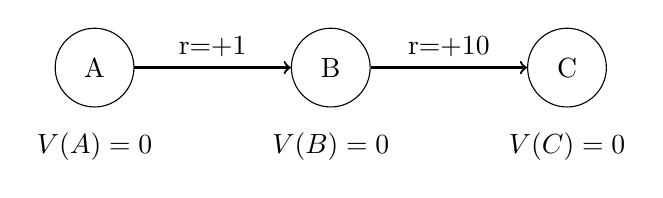
\begin{tikzpicture}[
            node distance=3cm,
            state/.style={circle, draw, minimum size=1cm}
        ]
            \node[state] (A) {A};
            \node[state, right of=A] (B) {B};
            \node[state, right of=B] (C) {C};

            \draw[->, thick] (A) -- (B) node[midway, above] {r=+1};
            \draw[->, thick] (B) -- (C) node[midway, above] {r=+10};

            \node at (0,-1) {$V(A)=0$};
            \node at (3,-1) {$V(B)=0$};
            \node at (6,-1) {$V(C)=0$};
        \end{tikzpicture}
    \end{center}
\end{frame}

\begin{frame}
    \frametitle{Step-by-Step TD Updates}

    \begin{block}<1->{Episode: A → B → C}
        Let's trace through one episode and see how values update:
    \end{block}

    \begin{block}<2->{Step 1: A → B (receive reward = +1)}
        \textcolor{tdmain}{\textbf{TD Update for A:}}
        \begin{align*}
            V(A) &= V(A) + \alpha[r + \gamma V(B) - V(A)]\\
            &= 0 + 0.5[1 + 0.9 \times 0 - 0]\\
            &= 0 + 0.5 \times 1 = \textcolor{red}{\mathbf{0.5}}
        \end{align*}
    \end{block}
\end{frame}

\begin{frame}
    \frametitle{Step-by-Step TD Updates}

    \begin{block}<1->{Episode: A → B → C}
        Let's trace through one episode and see how values update:
    \end{block}

    \begin{block}<2->{Step 2: B → C (receive reward = +10)}
        \textcolor{tdmain}{\textbf{TD Update for B:}}
        \begin{align*}
            V(B) &= V(B) + \alpha[r + \gamma V(C) - V(B)]\\
            &= 0 + 0.5[10 + 0.9 \times 0 - 0]\\
            &= 0 + 0.5 \times 10 = \textcolor{red}{\mathbf{5.0}}
        \end{align*}
    \end{block}
\end{frame}

\begin{frame}
    \frametitle{After First Episode}

    \begin{center}
        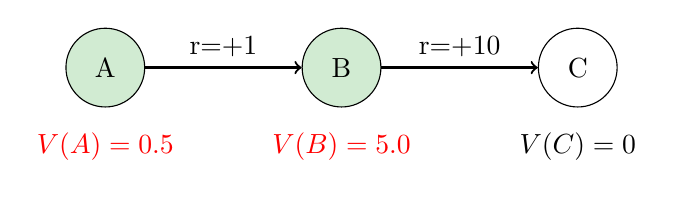
\begin{tikzpicture}[
            node distance=3cm,
            state/.style={circle, draw, minimum size=1cm}
        ]
            \node[state, fill=tdlight!30] (A) {A};
            \node[state, fill=tdlight!30, right of=A] (B) {B};
            \node[state, right of=B] (C) {C};

            \draw[->, thick] (A) -- (B) node[midway, above] {r=+1};
            \draw[->, thick] (B) -- (C) node[midway, above] {r=+10};

            \node at (0,-1) {\textcolor{red}{$V(A)=0.5$}};
            \node at (3,-1) {\textcolor{red}{$V(B)=5.0$}};
            \node at (6,-1) {$V(C)=0$};
        \end{tikzpicture}
    \end{center}
    \begin{block}<2->{Second Episode: A → B → C}
        \textcolor{tdmain}{\textbf{Now A uses updated V(B):}}
        \begin{align*}
            V(A) &\leftarrow 0.5 + 0.5[1 + 0.9 \times 5.0 - 0.5]\\
            &\leftarrow 0.5 + 0.5[1 + 4.5 - 0.5]\\
            &\leftarrow 0.5 + 0.5 \times 5.0 = \textcolor{red}{\mathbf{3.0}}
        \end{align*}
    \end{block}
    \begin{block}<3->{Key Insight}
        \textcolor{tdaccent}{\textbf{TD uses updated estimates}} - V(A) learned from V(B)'s improvement!
    \end{block}
\end{frame}

\begin{frame}
    \frametitle{Compare with Monte Carlo}

    \begin{columns}
        \begin{column}{0.48\textwidth}
            \begin{block}{\textcolor{blue}{Monte Carlo}}
                \begin{itemize}
                    \item<1-> Waits for complete episode
                    \item<2-> A gets return: $1 + 0.9 \times 10 = 10$
                    \item<3-> After episode 1: $V(A) = 5.0$
                    \item<4-> No learning until end
                \end{itemize}
            \end{block}
        \end{column}
        \begin{column}{0.48\textwidth}
            \begin{block}{\textcolor{tdmain}{TD Learning}}
                \begin{itemize}
                    \item<5-> Updates at each step
                    \item<6-> A uses estimate: $1 + 0.9 \times 0 = 1$
                    \item<7-> After step 1: $V(A) = 0.5$
                    \item<8-> Learns progressively
                \end{itemize}
            \end{block}
        \end{column}
    \end{columns}

    \begin{block}<9->{Why This Matters}
        \begin{itemize}
            \item<9-> TD starts learning \textcolor{tdaccent}{\textbf{immediately}}
            \item<10-> Values \textcolor{tdmain}{\textbf{propagate}} through the chain
            \item<11-> More robust to \textcolor{tderror}{\textbf{incomplete episodes}}
        \end{itemize}
    \end{block}
\end{frame}

\subsection{Example: Driving Time Prediction}

\begin{frame}
    \frametitle{Practical Example: Driving to Friend's House}

    \begin{block}<1->{Scenario}
        \begin{itemize}
            \item<1-> Predict travel time to friend's house
            \item<2-> Consider: time of day, weather, traffic, etc.
            \item<3-> Learn from experience over multiple trips
        \end{itemize}
    \end{block}

    \begin{center}
        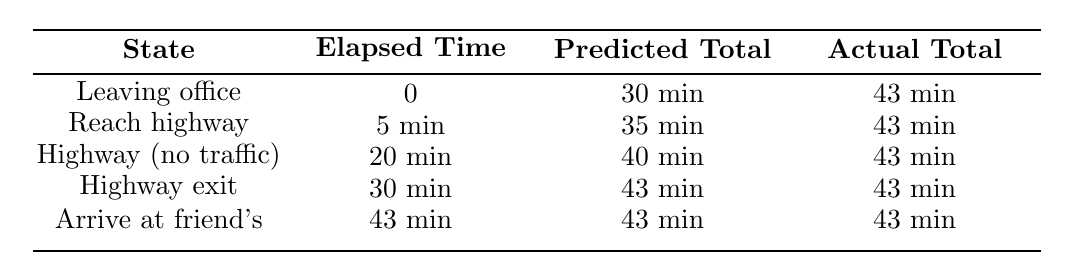
\begin{tikzpicture}[scale=0.8]
            % Table header
            \node at (0,2.7) {\textbf{State}};
            \node at (4,2.7) {\textbf{Elapsed Time}};
            \node at (8,2.7) {\textbf{Predicted Total}};
            \node at (12,2.7) {\textbf{Actual Total}};

            % Table rows
            \node at (0,2) {Leaving office};
            \node at (4,2) {0};
            \node at (8,2) {30 min};
            \node at (12,2) {43 min};

            \node at (0,1.5) {Reach highway};
            \node at (4,1.5) {5 min};
            \node at (8,1.5) {35 min};
            \node at (12,1.5) {43 min};

            \node at (0,1) {Highway (no traffic)};
            \node at (4,1) {20 min};
            \node at (8,1) {40 min};
            \node at (12,1) {43 min};

            \node at (0,0.5) {Highway exit};
            \node at (4,0.5) {30 min};
            \node at (8,0.5) {43 min};
            \node at (12,0.5) {43 min};

            \node at (0,0) {Arrive at friend's};
            \node at (4,0) {43 min};
            \node at (8,0) {43 min};
            \node at (12,0) {43 min};

            % Table lines
            \draw[thick] (-2,3) -- (14,3);
            \draw[thick] (-2,2.3) -- (14,2.3);
            \draw[thick] (-2,-0.5) -- (14,-0.5);
        \end{tikzpicture}
    \end{center}
\end{frame}

\begin{frame}
    \frametitle{MC vs TD Learning Comparison}

    \begin{columns}
        \begin{column}{0.6\textwidth}
            \begin{center}
                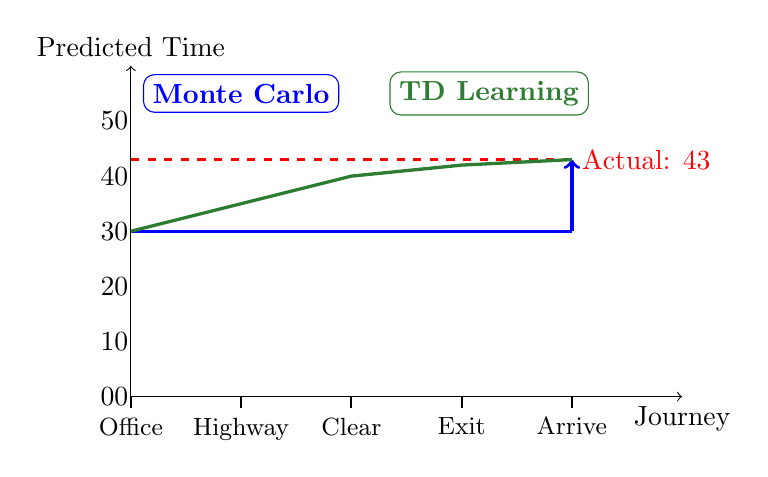
\begin{tikzpicture}[scale=0.7]
                    % Time axis
                    \draw[->] (0,0) -- (10,0) node[below] {Journey};
                    \draw[->] (0,0) -- (0,6) node[above] {Predicted Time};

                    % Y-axis labels
                    \foreach \y in {0,1,2,3,4,5}
                        \node at (-0.3,\y) {\y 0};

                    % Actual outcome line
                    \draw[thick, red, dashed] (0,4.3) -- (8,4.3) node[right] {\textcolor{red}{Actual: 43}};

                    % Monte Carlo - flat line then jump
                    \draw[very thick, blue] (0,3) -- (8,3);
                    \draw[very thick, blue, ->] (8,3) -- (8,4.3);

                    % TD Learning - step by step updates
                    \draw[very thick, tdmain] (0,3) -- (2,3.5) -- (4,4.0) -- (6,4.2) -- (8,4.3);

                    % State markers
                    \foreach \x/\label in {0/Office, 2/Highway, 4/Clear, 6/Exit, 8/Arrive}
                        \draw[thick] (\x,0) -- (\x,-0.2) node[below] {\small \label};

                    % Legend
                    \node[blue, fill=white, draw, rounded corners] at (2,5.5) {\textbf{Monte Carlo}};
                    \node[tdmain, fill=white, draw, rounded corners] at (6.5,5.5) {\textbf{TD Learning}};
                \end{tikzpicture}
            \end{center}
        \end{column}
        \begin{column}{0.38\textwidth}
            \begin{block}{Observations}
                \begin{itemize}
                    \item<1-> \textcolor{tdmain}{\textbf{TD}}: Updates prediction continuously during the trip
                    \item<2-> \textcolor{blue}{\textbf{MC}}: Only updates at the end of the trip
                    \item<3-> TD can \textcolor{tdlight}{\textbf{adapt}} to new information immediately
                    \item<4-> MC waits for \textcolor{red}{\textbf{complete}} episode
                \end{itemize}
            \end{block}
        \end{column}
    \end{columns}
\end{frame}

\begin{frame}
    \frametitle{Advantages of TD Learning}

    \begin{block}{Why TD Learning is Powerful}
        \begin{itemize}
            \item<1-> \textcolor{tdmain}{\textbf{Model-free}}: No need for environment model
            \item<2-> \textcolor{tdaccent}{\textbf{Online learning}}: Updates at every step
            \item<3-> \textcolor{tdlight}{\textbf{Fully incremental}}: Constant memory requirements
            \item<4-> \textcolor{tdsecondary}{\textbf{Bootstrapping}}: Learns from estimates
            \item<5-> \textcolor{tdvalue}{\textbf{Practical}}: Works in continuing tasks
        \end{itemize}
    \end{block}

    \begin{block}<6->{When to Use TD}
        \begin{itemize}
            \item<6-> When episodes are very long or infinite
            \item<7-> When you need \textcolor{tdaccent}{\textbf{real-time}} learning
            \item<8-> When computational resources are limited
        \end{itemize}
    \end{block}
\end{frame}

% Section: SARSA
\section{SARSA: On-Policy TD Control}

\subsection{From Prediction to Control}

\begin{frame}
    \frametitle{Moving to Control: Action-Value Functions}

    \begin{block}<1->{Why Action-Value Functions?}
        \begin{itemize}
            \item<1-> Need to estimate $q_\pi(s,a)$ for all states and actions
            \item<2-> Essential for \textcolor{tdmain}{\textbf{policy improvement}}
            \item<3-> Must balance \textcolor{tdaccent}{\textbf{exploration}} and \textcolor{tdsecondary}{\textbf{exploitation}}
        \end{itemize}
    \end{block}

    \begin{block}<4->{Activity}
        \textcolor{tdactivity}{\textbf{Why do we need state-action pairs instead of just states?}}
    \end{block}

    \begin{block}<5->{Answer}
        \begin{itemize}
            \item<5-> Need to know \textcolor{tdvalue}{\textbf{value of each action}} in each state
            \item<6-> Essential for \textcolor{tdimprove}{\textbf{policy improvement}}
            \item<7-> Cannot improve policy with only state values
        \end{itemize}
    \end{block}
\end{frame}

\begin{frame}
    \frametitle{SARSA Update Rule}

    \begin{block}<1->{From State Values to Action Values}
        Replace $V(s)$ with $Q(s,a)$ in the TD update:
    \end{block}

    \begin{block}<2->{SARSA Update}
        \begin{equation}
            Q(s_t,a_t) \leftarrow Q(s_t,a_t) + \alpha\left[ r_{t+1} + \gamma Q(s_{t+1}, a_{t+1}) - Q(s_t, a_t) \right]
        \end{equation}
    \end{block}
    Uses every element: $(s_t, a_t, r_{t+1}, s_{t+1}, a_{t+1})$
    \begin{itemize}
        \item<4-> State $s_t$
        \item<5-> Action $a_t$
        \item<6-> Reward $r_{t+1}$
        \item<7-> State $s_{t+1}$
        \item<8-> Action $a_{t+1}$
    \end{itemize}
\end{frame}

\subsection{SARSA Algorithm}

\begin{frame}
    \frametitle{SARSA Algorithm}

    \begin{algorithm}[H]
        \caption{SARSA}
        \begin{algorithmic}[1]
            \State \textbf{Inputs:} $N$ (episodes), $\alpha \in [0,1]$ (step size)
            \State \textbf{Initialize:} $Q(s,a) \in \mathbb{R}$ arbitrarily, $\forall s \in S, a \in A$, except $Q(terminal, \cdot) = 0$
            \For{$episode = 1$ to $N$}
                \State Initialize $s$
                \State $a \leftarrow$ action from $Q(s,\cdot)$ using $\epsilon$-greedy
                \While{$s \neq terminal$}
                    \State $r, s' \leftarrow$ Execute $a$
                    \State $a' \leftarrow$ action from $Q(s',\cdot)$ using $\epsilon$-greedy
                    \State $Q(s,a) \leftarrow Q(s,a) + \alpha[r + \gamma Q(s',a') - Q(s,a)]$
                    \State $s \leftarrow s'$, $a \leftarrow a'$
                \EndWhile
            \EndFor
        \end{algorithmic}
    \end{algorithm}
\end{frame}

\begin{frame}
    \frametitle{SARSA Key Properties}

    \begin{block}<1->{On-Policy Learning}
        \begin{itemize}
            \item<1-> Learns about the \textcolor{tdonpolicy}{\textbf{same policy}} it follows
            \item<2-> Both behavior and target policy use $\epsilon$-greedy
            \item<3-> Updates $Q(s,a)$ for the action actually taken
        \end{itemize}
    \end{block}

    \begin{block}<4->{Action Selection Strategy}
        \begin{itemize}
            \item<4-> Typically uses \textcolor{tdaccent}{\textbf{$\epsilon$-greedy}} policy
            \item<5-> Balances exploration and exploitation
            \item<6-> Other strategies can be used (softmax, UCB, etc.)
        \end{itemize}
    \end{block}

    \begin{block}<7->{Important Note}
        \textcolor{tdmain}{\textbf{No explicit policy is stored!}} The policy is \textcolor{tdaccent}{\textbf{implicit}} in the Q-values.
    \end{block}
\end{frame}

% Section: Q-Learning
\section{Q-Learning: Off-Policy TD Control}

\subsection{The Q-Learning Algorithm}

\begin{frame}
    \frametitle{Q-Learning: A Classic Algorithm}

    \begin{block}<1->{Historical Note}
        \begin{itemize}
            \item<1-> Introduced in \textbf{1989} by Chris Watkins
            \item<2-> One of the most important RL algorithms
            \item<3-> Foundation for many modern methods
        \end{itemize}
    \end{block}

    \begin{block}<4->{Q-Learning Update Rule}
        \begin{equation}
            Q(s_t,a_t) \leftarrow Q(s_t,a_t) + \alpha\left[ r_{t+1} + \gamma\max_{a'} Q(s_{t+1}, a') - Q(s_t, a_t) \right]
        \end{equation}
    \end{block}

    \begin{block}<5->{Key Difference from SARSA}
        \begin{itemize}
            \item<5-> Uses \textcolor{tdoffpolicy}{\textbf{$\max_{a'} Q(s_{t+1}, a')$}} instead of $Q(s_{t+1}, a_{t+1})$
            \item<6-> Approximates \textcolor{tdmain}{\textbf{$q^*$}} (optimal action-value function)
        \end{itemize}
    \end{block}
\end{frame}

\begin{frame}
    \frametitle{Q-Learning Algorithm}

    \begin{algorithm}[H]
        \caption{Q-Learning}
        \begin{algorithmic}[1]
            \State \textbf{Inputs:} $N$ (episodes), $\alpha \in [0,1]$ (step size)
            \State \textbf{Initialize:} $Q(s,a) \in \mathbb{R}$ arbitrarily, $\forall s \in S, a \in A$, except $Q(terminal, \cdot) = 0$
            \For{$episode = 1$ to $N$}
                \State Initialize $s$
                \While{$s \neq terminal$}
                    \State $a \leftarrow$ action from $Q(s,\cdot)$ using $\epsilon$-greedy
                    \State $r, s' \leftarrow$ Execute $a$
                    \State $Q(s,a) \leftarrow Q(s,a) + \alpha[r + \gamma \max_{a'} Q(s',a') - Q(s,a)]$
                    \State $s \leftarrow s'$
                \EndWhile
            \EndFor
        \end{algorithmic}
    \end{algorithm}
\end{frame}

\subsection{SARSA vs Q-Learning}

\begin{frame}
    \frametitle{Activity: Spot the Differences}

    \begin{block}{Question}
        \textcolor{tdactivity}{\textbf{What is the difference between SARSA and Q-Learning algorithms?}}
    \end{block}

    \pause

    \begin{block}{Key Differences}
        \begin{enumerate}
            \item<2-> \textbf{Policy Type}:
                \begin{itemize}
                    \item SARSA: \textcolor{tdonpolicy}{\textbf{On-policy}} (learns about policy it follows)
                    \item Q-Learning: \textcolor{tdoffpolicy}{\textbf{Off-policy}} (learns about optimal policy)
                \end{itemize}
            \item<3-> \textbf{Update Target}:
                \begin{itemize}
                    \item SARSA: $Q(s_{t+1}, a_{t+1})$ (actual next action)
                    \item Q-Learning: $\max_{a'} Q(s_{t+1}, a')$ (best possible action)
                \end{itemize}
            \item<4-> \textbf{Next Action Selection}:
                \begin{itemize}
                    \item SARSA: Needs $a_{t+1}$ before update
                    \item Q-Learning: No need for actual next action
                \end{itemize}
        \end{enumerate}
    \end{block}
\end{frame}

\begin{frame}
    \frametitle{On-Policy vs Off-Policy Behavior}

    \begin{columns}
        \begin{column}{0.48\textwidth}
            \begin{block}{SARSA (On-Policy)}
                \begin{itemize}
                    \item<1-> \textcolor{tdonpolicy}{\textbf{Conservative}}
                    \item<2-> Learns the value of the \textcolor{tdaccent}{\textbf{actual policy}} followed
                    \item<3-> Considers exploration in learning
                    \item<4-> Safer in dangerous environments
                \end{itemize}
            \end{block}
        \end{column}
        \begin{column}{0.48\textwidth}
            \begin{block}{Q-Learning (Off-Policy)}
                \begin{itemize}
                    \item<5-> \textcolor{tdoffpolicy}{\textbf{Optimistic}}
                    \item<6-> Learns the value of the \textcolor{tdmain}{\textbf{optimal policy}}
                    \item<7-> Ignores exploration in learning
                    \item<8-> Faster convergence to optimal
                \end{itemize}
            \end{block}
        \end{column}
    \end{columns}

    \begin{block}<9->{Practical Implications}
        \begin{itemize}
            \item<9-> \textbf{SARSA}: Better for \textcolor{tderror}{\textbf{risky}} environments (cliff walking)
            \item<10-> \textbf{Q-Learning}: Better for finding \textcolor{tdvalue}{\textbf{optimal}} policies
        \end{itemize}
    \end{block}
\end{frame}

\begin{frame}
    \frametitle{Visual Comparison: Update Mechanisms}

    \begin{center}
        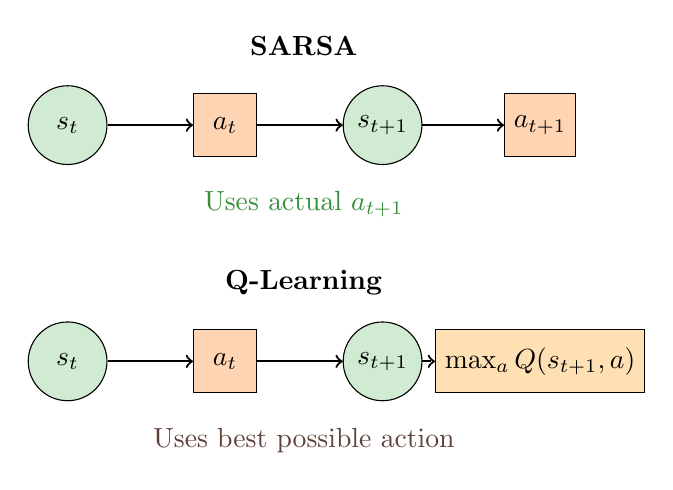
\begin{tikzpicture}[
            node distance=2cm,
            state/.style={circle, draw, minimum size=1cm},
            action/.style={rectangle, draw, minimum size=0.8cm}
        ]
            % SARSA
            \node[state, fill=tdlight!30] (s1) at (0,2) {$s_t$};
            \node[action, fill=tdaccent!30] (a1) at (2,2) {$a_t$};
            \node[state, fill=tdlight!30] (s2) at (4,2) {$s_{t+1}$};
            \node[action, fill=tdaccent!30] (a2) at (6,2) {$a_{t+1}$};

            \draw[->, thick] (s1) -- (a1);
            \draw[->, thick] (a1) -- (s2);
            \draw[->, thick] (s2) -- (a2);

            \node at (3,3) {\textbf{SARSA}};
            \node at (3,1) {\textcolor{tdonpolicy}{Uses actual $a_{t+1}$}};

            % Q-Learning
            \node[state, fill=tdlight!30] (s3) at (0,-1) {$s_t$};
            \node[action, fill=tdaccent!30] (a3) at (2,-1) {$a_t$};
            \node[state, fill=tdlight!30] (s4) at (4,-1) {$s_{t+1}$};
            \node[action, fill=tdvalue!30] (a4) at (6,-1) {$\max_a Q(s_{t+1},a)$};

            \draw[->, thick] (s3) -- (a3);
            \draw[->, thick] (a3) -- (s4);
            \draw[->, thick, dashed] (s4) -- (a4);

            \node at (3,0) {\textbf{Q-Learning}};
            \node at (3,-2) {\textcolor{tdoffpolicy}{Uses best possible action}};
        \end{tikzpicture}
    \end{center}
\end{frame}

% Section: Summary
\section{Summary}

\subsection{TD Learning Advantages}

\begin{frame}
    \frametitle{Why TD Learning Matters}

    \begin{block}<1->{Core Advantages}
        \begin{itemize}
            \item<1-> \textcolor{tdmain}{\textbf{Model-free}}: No environment model required
            \item<2-> \textcolor{tdaccent}{\textbf{Online}}: Learn during interaction
            \item<3-> \textcolor{tdlight}{\textbf{Incremental}}: Constant memory and computation
            \item<4-> \textcolor{tdsecondary}{\textbf{Bootstrapping}}: Faster than Monte Carlo
        \end{itemize}
    \end{block}

    \begin{block}<5->{Practical Benefits}
        \begin{itemize}
            \item<5-> Works with \textcolor{tdvalue}{\textbf{continuing tasks}}
            \item<6-> Suitable for \textcolor{tdaccent}{\textbf{real-time}} applications
            \item<7-> Foundation for \textcolor{tdmain}{\textbf{modern deep RL}}
        \end{itemize}
    \end{block}
\end{frame}

\begin{frame}
    \frametitle{Method Comparison Summary}

    \begin{center}
        \begin{tabular}{|l|c|c|c|c|}
            \hline
            \textbf{Method} & \textbf{Model-Free} & \textbf{Online} & \textbf{Policy Type} & \textbf{Convergence} \\
            \hline
            \rowcolor{gray!20}
            Monte Carlo & \textcolor{green}{Yes} & \textcolor{red}{No} & On/Off & Guaranteed \\
            \hline
            \rowcolor{tdlight!30}
            \textbf{TD(0)} & \textcolor{green}{\textbf{Yes}} & \textcolor{green}{\textbf{Yes}} & \textbf{On} & \textbf{Guaranteed} \\
            \hline
            \rowcolor{tdonpolicy!30}
            \textbf{SARSA} & \textcolor{green}{\textbf{Yes}} & \textcolor{green}{\textbf{Yes}} & \textbf{On} & \textbf{Guaranteed} \\
            \hline
            \rowcolor{tdoffpolicy!30}
            \textbf{Q-Learning} & \textcolor{green}{\textbf{Yes}} & \textcolor{green}{\textbf{Yes}} & \textbf{Off} & \textbf{Guaranteed} \\
            \hline
        \end{tabular}
    \end{center}

    \begin{block}<2->{When to Use Each}
        \begin{itemize}
            \item<2-> \textbf{SARSA}: Safe exploration, learns about followed policy
            \item<3-> \textbf{Q-Learning}: Optimal policies, faster convergence
            \item<4-> Both: Foundation for function approximation methods
        \end{itemize}
    \end{block}
\end{frame}

\begin{frame}
    \frametitle{Key Takeaways}

    \begin{block}<1->{Fundamental Concepts}
        \begin{itemize}
            \item<1-> \textcolor{tdmain}{\textbf{TD Error}}: Measures prediction accuracy
            \item<2-> \textcolor{tdaccent}{\textbf{Bootstrapping}}: Learn from estimates
            \item<3-> \textcolor{tdsecondary}{\textbf{Online Learning}}: Update at every step
        \end{itemize}
    \end{block}

    \begin{block}<4->{Algorithm Choice}
        \begin{itemize}
            \item<4-> Use \textcolor{tdonpolicy}{\textbf{SARSA}} when safety matters
            \item<5-> Use \textcolor{tdoffpolicy}{\textbf{Q-Learning}} for optimal performance
            \item<6-> Both are \textcolor{tdvalue}{\textbf{foundations}} for advanced methods
        \end{itemize}
    \end{block}

    \begin{block}<7->{Next Steps}
        \begin{itemize}
            \item<7-> Function approximation (Deep Q-Networks)
            \item<8-> Policy gradient methods
            \item<9-> Actor-Critic algorithms
        \end{itemize}
    \end{block}
\end{frame}

\begin{frame}
    \frametitle{Questions?}

    \begin{center}
        \Huge \textcolor{tdmain}{\textbf{Questions?}}

        \vspace{2em}

        \Large Thank you for your attention!

        \vspace{1em}

        \normalsize
        Next: Function Approximation Methods
    \end{center}
\end{frame}

\end{document}
